\documentclass{article}
\usepackage[utf8]{inputenc}
\usepackage[spanish,mexico]{babel}
\usepackage{csquotes}
\usepackage{caption}
\usepackage{enumitem}
\usepackage{geometry}
\usepackage{mathtools}
\usepackage{multicol}
\usepackage[backend=bibtex]{biblatex}
\usepackage{graphicx}
\usepackage{fancyvrb}
\usepackage{float}
\usepackage{hyperref}
\usepackage{numprint}

\addbibresource{references.bib}

 \geometry{
 %total={170mm,257mm},
 top=20mm,
 bottom=20mm,
 left=20mm,
 right=20mm
 }
 
 \graphicspath{{./img/}}

\title{\textbf{Arquitectura de Computadoras} \\ 
Organización de caché y evaluación de desempeño}
\author{Mario Becerra \\ Luis Daniel Hernández}
\date{Marzo de 2017}

\setlength\parindent{0pt}
\setlength{\parskip}{0.5em}

\begin{document}
\npthousandsep{,}

\maketitle

\section{Introducción}

%%%%%%%%%%%%%%%%%%%%%%%%%%%%%%%%%%%%%%%%%%%%%%%%%%%%%%%%%%%%%%%%%%%%%%%%
%%%%%%%%%%%%%%%%%%%%%%%%%%%%%%%%%%%%%%%%%%%%%%%%%%%%%%%%%%%%%%%%%%%%%%%%
%%%%%%%% INTRODUCCIÓN
%%%%%%%%%%%%%%%%%%%%%%%%%%%%%%%%%%%%%%%%%%%%%%%%%%%%%%%%%%%%%%%%%%%%%%%%
%%%%%%%%%%%%%%%%%%%%%%%%%%%%%%%%%%%%%%%%%%%%%%%%%%%%%%%%%%%%%%%%%%%%%%%%

En esta práctica se implementa un simulador de caché basado en trazas con el objetivo de reforzar la teoría vista en clase sobre cómo funcionan los cachés. Con el simulador implementado, se analizan distintas configuraciones de caché, las cuales también fueron discutidas en clase.

El simulador toma como entrada una serie de lecturas y escrituras a memoria, las cuales fueron proporcionados por el profesor. El simulador es configurable y se le puede modificar las características de tamaño de caché, de tamaño de bloque, si es un caché unificado o separado por instrucciones y datos (I-D), políticas de escritura \textit{write-back}, \textit{write-through}, \textit{write-allocate} o \textit{write-no-allocate}. El simulador rastrea el número de referencias de instrucciones y de datos, número de \textit{misses} de datos y de instrucciones, número de palabras adquiridas de memoria y número de palabras escritas en memoria. En los casos en que la asociatividad es mayor a 1, la política de reemplazo utilizada es \textit{Least-Recently-Used} (LRU).



\section{Marco teórico}

%%%%%%%%%%%%%%%%%%%%%%%%%%%%%%%%%%%%%%%%%%%%%%%%%%%%%%%%%%%%%%%%%%%%%%%%
%%%%%%%%%%%%%%%%%%%%%%%%%%%%%%%%%%%%%%%%%%%%%%%%%%%%%%%%%%%%%%%%%%%%%%%%
%%%%%%%% MARCO TEÓRICO
%%%%%%%%%%%%%%%%%%%%%%%%%%%%%%%%%%%%%%%%%%%%%%%%%%%%%%%%%%%%%%%%%%%%%%%%
%%%%%%%%%%%%%%%%%%%%%%%%%%%%%%%%%%%%%%%%%%%%%%%%%%%%%%%%%%%%%%%%%%%%%%%%

Se espera que el lector de este trabajo est\'e familiarizado con la funcionalidad de un caché y sus tecnicismos. Sin embargo, a continuación se mencionan y explican algunos de los conceptos más utilizados en este trabajo.

Un caché unificado es uno en el que se guardan instrucciones y datos, mientras que un caché I-D es uno en el que en realidad se tienen dos cachés: uno para instrucciones y uno para datos; todas las referencias que tienen que ver con datos se hacen con el caché D, mientras que todas las que tienen que ver con instrucciones se hacen con el caché I.

Las políticas de escritura \textit{write-back} y \textit{write-through} se establecen para cuando se tiene un \textit{hit} en una referencia a escritura de un dato. En la política \textit{write-through} se escribe la palabra en caché y en memoria, mientras que en \textit{write-back} se escribe solo en caché, por lo cual se tiene un \textit{dirty bit} que indica si el bloque de memoria es inconsistente con el bloque que está en caché.

Análogamente, las políticas de escritura \textit{write-allocate} y \textit{write-no-allocate} se establecen para cuando se tiene un \textit{miss} en una referencia de escritura. En el caso de \textit{write-allocate}, se trae a caché el bloque en el que se encuentra la localidad de memoria en la cual se quiere escribir para después modificar la memoria únicamente en el caché. Por el contrario, en la política \textit{write-no-allocate}, se escribe únicamente en la memoria principal.

Usualmente, las combinaciones que se utilizan son \textit{write-back} con \textit{write-allocate} y \textit{write-through} con \textit{write-no-allocate}.

La política de reemplazo LRU es de la siguiente forma: cuando se tiene una colisión en un \textit{set}, si todas las páginas de ese \textit{set} están ocupadas, se reemplaza la página que fue usada hace más tiempo. Para poder implementar esta política, se tiene que saber en todo momento el orden en que han sido utilizadas las páginas. En el caso de esta práctica se hace con una lista doblemente ligada en la cual se elimina la cola cuando hay que reemplazar, y cada vez que se accede a una página, se pone en la cabeza de la lista para que así en la cabeza siempre esté la página que se usó más recientemente y en la cola la que menos.





\section{Evaluación de desempeño}

%%%%%%%%%%%%%%%%%%%%%%%%%%%%%%%%%%%%%%%%%%%%%%%%%%%%%%%%%%%%%%%%%%%%%%%%
%%%%%%%%%%%%%%%%%%%%%%%%%%%%%%%%%%%%%%%%%%%%%%%%%%%%%%%%%%%%%%%%%%%%%%%%
%%%%%%%% EVALUACIÓN DE DESEMPEÑO
%%%%%%%%%%%%%%%%%%%%%%%%%%%%%%%%%%%%%%%%%%%%%%%%%%%%%%%%%%%%%%%%%%%%%%%%
%%%%%%%%%%%%%%%%%%%%%%%%%%%%%%%%%%%%%%%%%%%%%%%%%%%%%%%%%%%%%%%%%%%%%%%%

En esta sección se evalúa el desempeño para cada uno de los archivos de trazas indicados, como función de distintos parámetros, manteniendo todo lo demás constante. Se presenta una gráfica para cada archivo, y en cada gráfica se muestran los resultados para el caché de datos (D) y el de instrucciones (I).


\subsection{Tamaño de caché}

%%%%%%%%%%%%%%%%%%
%% Tamaño de caché
%%%%%%%%%%%%%%%%%%

En esta subsección, se analiza el desempeño como función del tamaño. Se utiliza un caché \textit{full-associative} con un tamaño de bloque de 4 bytes, políticas de escritura \textit{write-back} y \textit{write-allocate}. En la figura \ref{fig:1_wsc} se puede ver la tasa de \textit{hit} en el eje $y$ como función del tamaño en el eje $x$. Este eje está en escala logarítmica con base 2 y va desde 4 hasta \numprint{1073741824} bytes. Se puede ver que conforme aumenta el tamaño del caché, aumenta la tasa de \textit{hit}, esto debido a que mientras más grande es el caché, mayor es la probabilidad de que contenga al dato que se necesita; sin embargo, se llega a una asíntota en el 1 en la cual no importa cuánto aumente el tamaño, la tasa de \textit{hit} ya llegó al máximo. El punto en el que la tasa de \textit{hit} llega al máximo varía según el programa y según si se trata de instrucciones o de datos.

\begin{figure}[H]
    \centering
    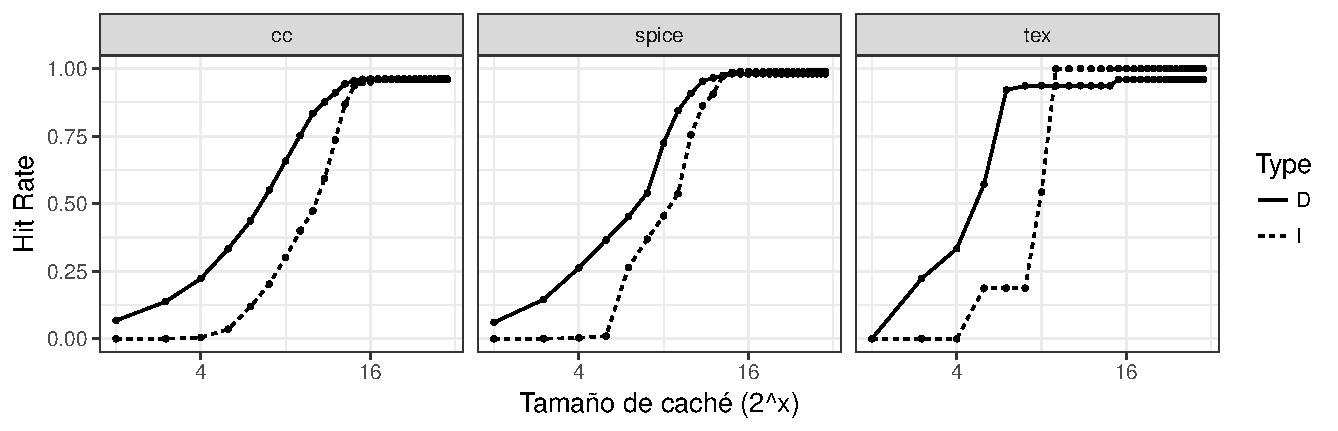
\includegraphics[width=\textwidth]{1_wsc.pdf}
    \caption{Tamaño de caché}
    \label{fig:1_wsc}
\end{figure}

En \cite{drepper2010every} mencionan que el \textit{working set size} es la cantidad total de memoria utilizada en cierto momento. En este caso, si se quisiera saber el \textit{working set size} de cada programa, se tendría que ver el archivo de trazas y contar el número de localidades de memoria utilizadas. En la tabla \ref{tab:num_loc_mem} se muestran estos números: distinguiendo si el tipo de acceso a memoria es de instrucción (I) o dato (D), y además se muestra el número de localidades únicas en cada caso. Cada localidad de memoria es de 32 bits, es decir, 4 bytes, por lo que si se quisiera saber el tamaño en bytes, se tendría que multiplicar el número de la tabla por 4.


\begin{table}[H]
    \centering
    \caption{Número de localidades de memoria utilizadas en cada archivo para accesos a datos (D) o instrucciones (I).}
    \label{tab:num_loc_mem}
    \begin{tabular}{|l|l|l|l|}
        \hline
        Archivo & Tipo & Localidades únicas & Localidades totales \\ \hline
        \texttt{cc}      & D    & \numprint{11856}              & \numprint{242661}              \\ \hline
        \texttt{cc}      & I    & \numprint{31195}              & \numprint{757341}              \\ \hline
        \texttt{spice}   & D    & \numprint{6356}               & \numprint{217237}              \\ \hline
        \texttt{spice}   & I    & \numprint{8964}               & \numprint{782764}              \\ \hline
        \texttt{tex}     & D    & \numprint{38026}              & \numprint{235168}              \\ \hline
        \texttt{tex}     & I    & \numprint{160}                & \numprint{597309}              \\ \hline
    \end{tabular}
\end{table}



\subsection{Impacto del Tamaño del Bloque}

%%%%%%%%%%%%%%%%%%
%% Tamaño de bloque
%%%%%%%%%%%%%%%%%%

% \begin{verbatim}
% $./sim -is 8192 -ds 8192 -bs 4,8,..,4096 -a 2 -wb -wa trazas/spice.trace >> spice_stats.txt
% $./sim -is 8192 -ds 8192 -bs 4,8,..,4096 -a 2 -wb -wa trazas/tex.trace >> tex_stats.txt
% $./sim -is 8192 -ds 8192 -bs 4,8,..,4096 -a 2 -wb -wa trazas/cc.trace >> cc_stats.txt
% \end{verbatim}

Ahora se analiza el desempeño dependiendo del tamaño del bloque. En este caso, se utilizó un caché de datos y uno de instrucciones de tamaño 8K-bytes cada uno, asociatividad 2 y políticas de escritura \textit{write-back} y \textit{write-allocate}. En la figura \ref{fig:2_block_size} se muestra la tasa de \textit{hit} como función del tamaño del bloque, el cual va desde 4 bytes hasta 4 K-bytes. Se observa que en un principio, con mayor tamaño de bloque se tiene mayor tasa de \textit{hit}, pero que esta tasa disminuye después de cierto punto. Esta disminución es más evidente en el caso del caché de datos, en el cual la tasa de \textit{hit} disminuye drásticamente a partir de más o menos el tamaño 128 para los tres archivos. La forma de esta curva tiene una razón sencilla, y esta es la del principio de localidad espacial, el cual dice que las instrucciones van a estar en localidades de memoria cercanas entre ellas debido a que se tienen instrucciones secuenciales y pocos saltos, además de variables agrupadas en los mismos bloques de memoria (por ejemplo, los arreglos). Debido a este principio, si se aumenta el tamaño de bloque, se cargan más localidades de memoria que van a ser utilizadas; pero si el tamaño del bloque es muy grande, al tener un tamaño fijo de caché, bloques más grandes implican menos \textit{sets} en un mismo caché, por lo cual se tienen que hacer más reemplazos.

En el caso de este simulador con el tamaño de caché que se utiliza, el tamaño óptimo de bloque para cada archivo sería:

\begin{itemize}
    \item \texttt{cc}: Para el caché de datos un tamaño de 32, y para el de instrucciones de 2048.
    \item \texttt{spice}: Para el caché de datos un tamaño de 32, y para el de instrucciones de 512 o 1024.
    \item \texttt{tex}: Para el caché de datos un tamaño de 128, y para el de instrucciones de 32 a 2048 (todos tienen tasa de \textit{hit} igual a 1).
\end{itemize}


\begin{figure}[H]
    \centering
    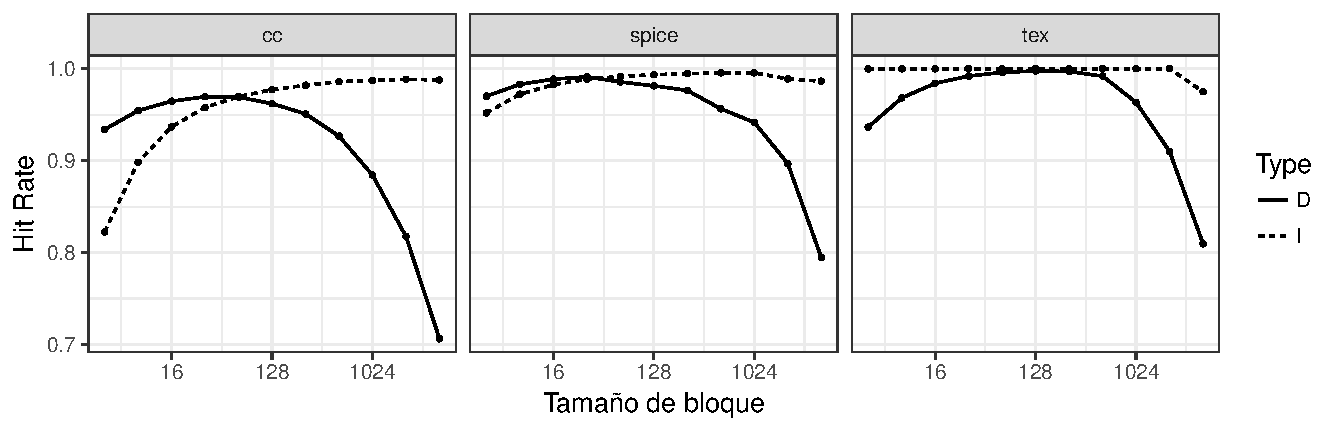
\includegraphics[width=\textwidth]{2_block_size.pdf}
    \caption{Tamaño de bloque}
    \label{fig:2_block_size}
\end{figure}





\subsection{Impacto de la Asociatividad}

%%%%%%%%%%%%%%%%%%
%% Asociatividad
%%%%%%%%%%%%%%%%%%

% \begin{verbatim}
% $./sim -is 8192 -ds 8192 -bs 128 -a 1,2,...,64 -wb -wa trazas/spice.trace >> spice_stats_assoc.txt
% $./sim -is 8192 -ds 8192 -bs 128 -a 1,2,...,64 -wb -wa trazas/tex.trace >> tex_stats_assoc.txt
% $./sim -is 8192 -ds 8192 -bs 128 -a 1,2,...,64 -wb -wa trazas/cc.trace >> cc_stats_assoc.txt    
% \end{verbatim}

En esta subsección se analiza el impacto que tiene la asociatividad en la tasa de \textit{hit}. Para este análisis se simula un caché I-D de 8K cada uno con tamaño de bloque de 128 con políticas de \textit{write-back} y \textit{write-allocate}. En la figura \ref{fig:3_assoc_size} se muestran las tasas de \textit{hit} como función de la asociatividad. En todos los casos, se puede ver que aumentar la asociatividad aumenta la tasa de \textit{hit}. El tener mayor asociatividad mejora la tasa de \textit{hit} siempre porque se tienen menos colisiones, por lo que hay menos reemplazos y menos \textit{misses}. Esto, naturalmente, viene con un costo, el cual es el de tener que buscar en todos las páginas de una misma línea para encontrar el \textit{tag} correspondiente al bloque de memoria en que se encuentra la palabra a la cual se quiere acceder.

Se puede apreciar que casi siempre la tasa de \textit{hit} es mayor en el caché de instrucciones que en el de datos, a excepción de \texttt{spice} a partir de asociatividad 4, sin embargo, estas diferencias se van haciendo más chicas conforme aumenta la asociatividad. 

\begin{figure}[H]
    \centering
    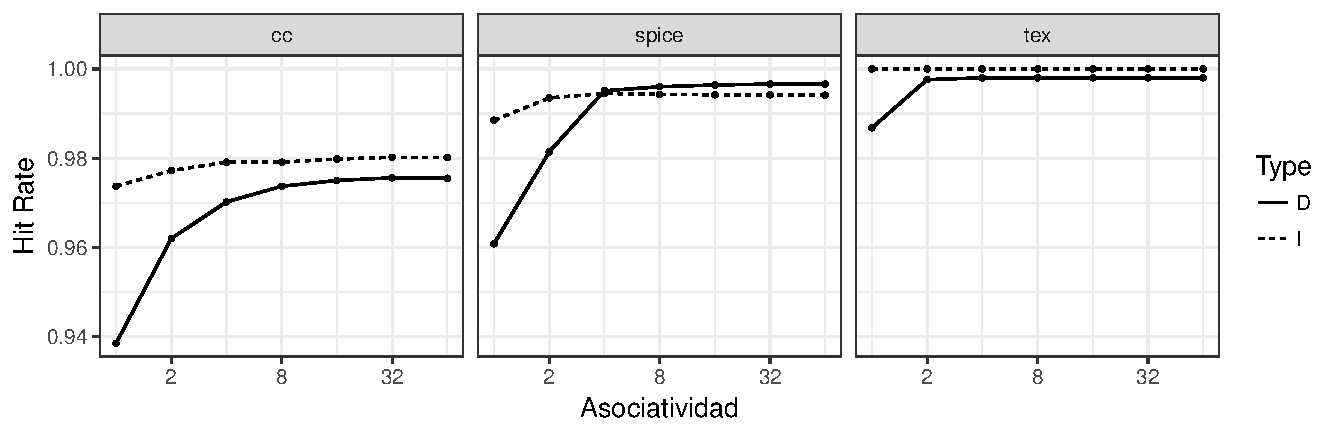
\includegraphics[width=\textwidth]{3_assoc_size.pdf}
    \caption{Asociatividad}
    \label{fig:3_assoc_size}
\end{figure}









\subsection{Ancho de Banda en Memoria}

%%%%%%%%%%%%%%%%%%
%% Ancho de banda de memoria
%%%%%%%%%%%%%%%%%%

En las figuras \ref{fig:4_memory_bandwidth_cc}, \ref{fig:4_memory_bandwidth_spice} y \ref{fig:4_memory_bandwidth_tex} se muestra la cantidad de \textit{copies back} y \textit{demand fetches} en un caché I-D simulado, para cada uno de los archivos. Cada figura corresponde a un archivo diferente, y cada cuadrante de la figura corresponde a una configuración de tamaño de caché y tamaño de bloque, y a su vez, cada subcuadrante corresponde al número de \textit{copies back} y de \textit{demand fetches} con política de escritura \textit{write-back} (WB) o \textit{write-through} (WT). Dentro de cada subcuadrante hay dos barras, cada una de las cuales corresponde a política \textit{write-allocate} (WA) o \textit{no-write-allocate} (NW).

Se puede ver que para el mismo tamaño de bloque, de caché y la misma asociatividad, la política de \textit{write-back} tiene exactamente el mismo número de \textit{demand fetches} que la política de \textit{write-through}; sin embargo, el número de \textit{copies back} es menor con la política de \textit{write-back}. Estas dos observaciones tienen razones: la razón de la primera es bastante simple, y es que la operación de \textit{demand fetch}, al ser una operación de \textbf{lectura}, no es afectada por la política de \textbf{escritura}, y por esto los números son iguales; la razón de la segunda observación es que en el caso de un \textit{hit}, con la política \textit{write-through} se tiene que escribir en la memoria principal en cada operación de escritura, mientras que en la política \textit{write-back} se escribe solamente en el caché, por lo que se reduce el número de accesos a memoria para escribir, es decir, los \textit{copies back}. Estos números podrían voltearse, i.e. que el número de \textit{copies back} fuera mayor en \textit{write-back} que en \textit{write-through}, si se ejecutara un programa en el que se la mayoría de las operaciones fueran de escritura en oposición a las de lectura.

Similarmente al caso anterior, para el mismo tamaño de bloque, de caché y la misma asociatividad, las políticas \textit{write-allocate} y \textit{write-no-allocate} tienen exactamente el mismo número de \textit{copies-back} si se sigue la política \textit{write-through}, pero con \textit{write-back}, no se ve un patrón claro del número de \textit{copies back}. En el caso de los \textit{demand fetches}, en todos los casos el valor de la política \textit{write-allocate} es mayor que el de \textit{write-no-allocate}, esto porque en el caso de \textit{miss}, la política \textit{write-allocate} trae todo un bloque de memoria a caché para luego escribir en este, mientras que \textit{write-no-allocate} solo escribe la palabra directamente en memoria; por lo que se tienen muchos más \textit{demand fetches}.

\begin{figure}[H]
    \centering
    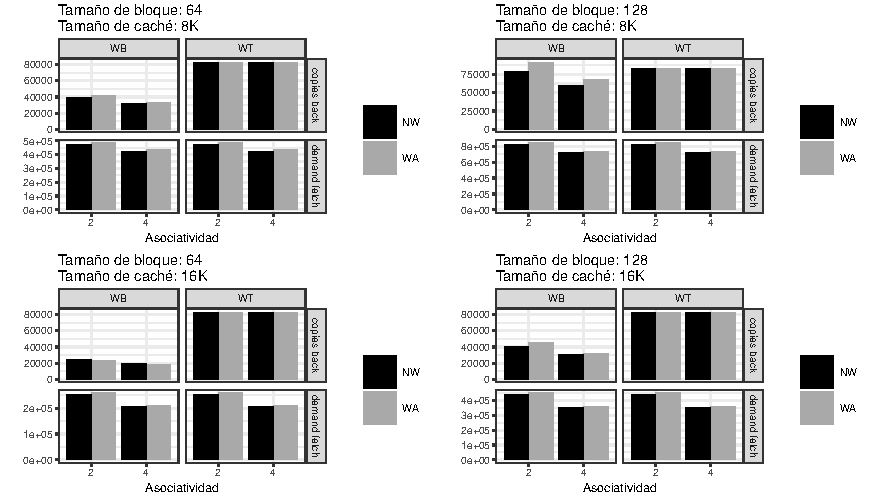
\includegraphics[width=\textwidth]{4_memory_bandwidth_wna_wa_cc.pdf}
    \caption{Cantidad de \textit{copies back} y \textit{demand fetches} para archivo \texttt{cc}.}
    \label{fig:4_memory_bandwidth_cc}
\end{figure}

\begin{figure}[H]
\centering
    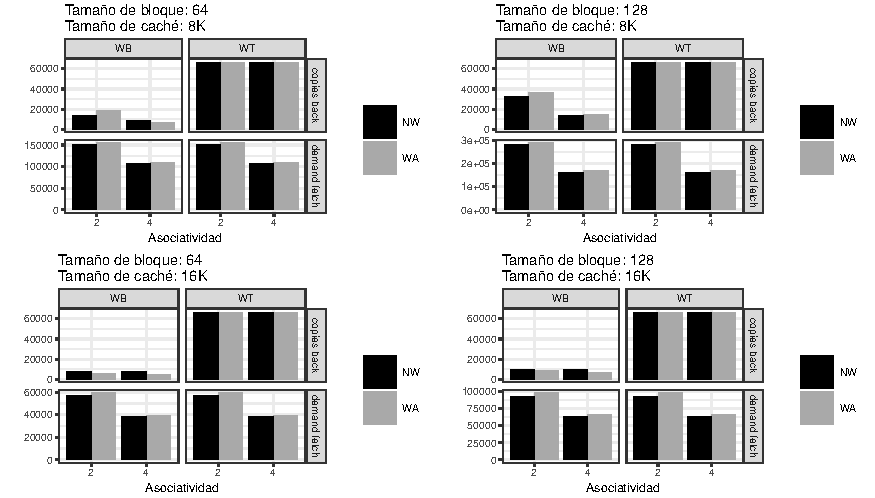
\includegraphics[width=\textwidth]{4_memory_bandwidth_wna_wa_spice.pdf}
    \caption{Cantidad de \textit{copies back} y \textit{demand fetches} para archivo \texttt{spice}.}
    \label{fig:4_memory_bandwidth_spice}
\end{figure}

\begin{figure}[H]
    \centering
    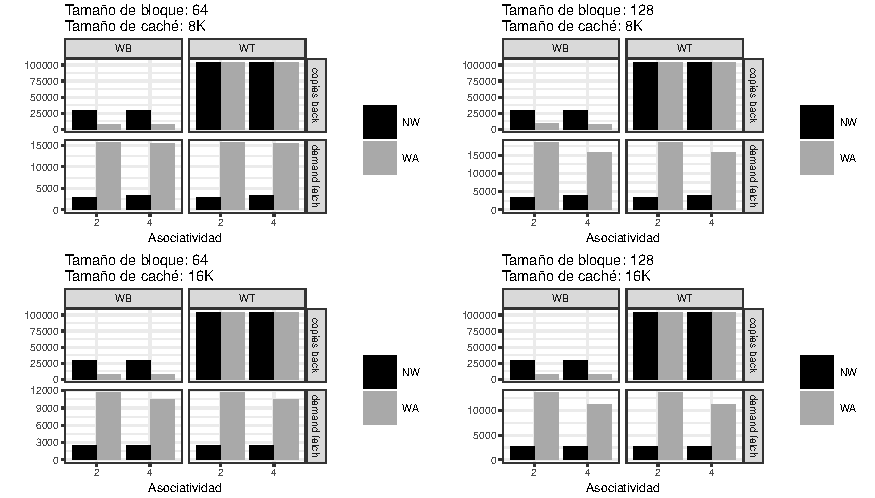
\includegraphics[width=\textwidth]{4_memory_bandwidth_wna_wa_tex.pdf}
    \caption{Cantidad de \textit{copies back} y \textit{demand fetches} para archivo \texttt{tex}.}
    \label{fig:4_memory_bandwidth_tex}
\end{figure}















\section{Conclusiones}

%%%%%%%%%%%%%%%%%%%%%%%%%%%%%%%%%%%%%%%%%%%%%%%%%%%%%%%%%%%%%%%%%%%%%%%%
%%%%%%%%%%%%%%%%%%%%%%%%%%%%%%%%%%%%%%%%%%%%%%%%%%%%%%%%%%%%%%%%%%%%%%%%
%%%%%%%% CONCLUSIONES
%%%%%%%%%%%%%%%%%%%%%%%%%%%%%%%%%%%%%%%%%%%%%%%%%%%%%%%%%%%%%%%%%%%%%%%%
%%%%%%%%%%%%%%%%%%%%%%%%%%%%%%%%%%%%%%%%%%%%%%%%%%%%%%%%%%%%%%%%%%%%%%%%

Este proyecto fue una buena experiencia para entender cómo funciona la memoria caché y reforzar los conceptos vistos en clase. Sin embargo, se tiene una curva de aprendizaje un tanto profunda con los archivos iniciales y, en particular, con la programación en C. Aún así, la práctica fue una experiencia enriquecedora llena de aprendizaje, con sus momentos de alta frustración.






\printbibliography
\nocite{*}


\end{document}
